\documentclass[12pt]{article}

\usepackage[margin=1in]{geometry}
\usepackage{amsmath,amsthm,amssymb}

\usepackage{graphicx}
\graphicspath{ {./assets/} }

\usepackage{algpseudocode}
\usepackage{algorithm}

\usepackage{tikz}

\newcommand{\wip}{\textbf{(WIP) }}
\newcommand{\tba}{\textbf{(TBA) }}

\newcommand{\blah}{\textbf{blah blah blah}}

\newcommand{\dsa}[1]{\textbf{[DSA: #1]}}

\begin{document}

\title{Project 1 - Report}
\author{
  Diogo Antunes\\
  99210
  \and
  Javier María\\
  99240
  \and
  Tomás Silva\\
  98973
}

\maketitle

\section*{\tba Exercise 1}

\section*{\wip Exercise 2}

% Instructions:
%   - Should include the encoding of the nonogram problem as a SAT problem
% Structure:
% - Two encodings were implemented
% - High-level overview of the encodings
%     - they share some of the structure (of encoding line by line)
%       - explain how this works
%       - In the following sections, we'll only talk about this simplified problem
%     - we have a brute force one that is easier to believe the correctness of but that (has complexity X)
%     - we have a more efficient one that is more complex but also uses less variables (has complexity Y)
%     - from the debugging standpoint, having both implementations proved useful because we were able to use one
% of the implementations to debug the other.
% - ``Brute-force'' approach
%   - One way is to consider all possible combinations
% - Polynomial approach
%   - Intuitively, a brute-force approach doesn't sound right
% - Experimental evaluation
%   - To understand what actually was better, we ran some benchmarks
%   - Show benchmarks, and comment on growth of brute-force approach

Two different encodings for the nonogram problem where implemented and tested.
Both encodings follow the same structure -- encoding the entire problem is reduced to encoding a single line with restrictions.
The encoding of the entire problem is just the and of the encodings of all rows and columns.
Let a line be a list of naturals, which denote the gaps that should exist in the line -- $l = [g_j, ..., g_{j'}]$.
A puzzle is a tuple $\langle H, V\rangle$, where both $H$ and $V$ a list of lines.
The propositional formula that is the encoding of a line $l = [g_j, ..., g_{j'}]$ of size $s$ will be denoted $E(l, s)$.
The two approaches will differ precisely on how $E$ is defined.
The encoding of the entire puzzle is

\begin{center}
  $\bigwedge\limits_{l \in H} E(l, |V|) \wedge \bigwedge\limits_{l \in V} E(l, |H|)$
\end{center}

Both approaches will be a variable per cell in the grid (but one of them will have more variables). The variable for cell at row $i$ and column $j$ will be denoted $x_i_j$.
At a high-level the first encoding uses a ``brute-force'' approach to solving the problem, by considering all possible placements of black regions in a given line.
The second approach tries to avoid this by encoding directly the dependencies between black regions and the rules of the game.
Having both approaches proved useful -- the brute-force one was easy to reason about and was used to debug the second approach.
In the following sub-sections, we will look in detail at how each encoding is made.

\subsection*{``Brute-force'' approach}

As hinted at before, the first and simpler approach to encoding the constraints for a single line is to consider all possible placements of segments of the specified sizes on the line.
For instance, if $l = [1, 2]$ for a line of size 5, the possible configurations are the following:

\begin{center}

\begin{tikzpicture}
    % X _ X X _
    \foreach \x in {1,2,...,5} {
        \ifnum\x=1 \filldraw[fill=black] (\x*0.5, 0) rectangle (\x*0.5+0.5, -0.5);
        \else\ifnum\x=3 \filldraw[fill=black] (\x*0.5, 0) rectangle (\x*0.5+0.5, -0.5);
        \else\ifnum\x=4 \filldraw[fill=black] (\x*0.5, 0) rectangle (\x*0.5+0.5, -0.5);
        \else \draw (\x*0.5, 0) rectangle (\x*0.5+0.5, -0.5);
        \fi\fi\fi
    }

    % X _ _ X X
    \begin{scope}[shift={(3.5, 0)}]
    \foreach \x in {1,2,...,5} {
        \ifnum\x=1 \filldraw[fill=black] (\x*0.5, 0) rectangle (\x*0.5+0.5, -0.5);
        \else\ifnum\x=4 \filldraw[fill=black] (\x*0.5, 0) rectangle (\x*0.5+0.5, -0.5);
        \else\ifnum\x=5 \filldraw[fill=black] (\x*0.5, 0) rectangle (\x*0.5+0.5, -0.5);
        \else \draw (\x*0.5, 0) rectangle (\x*0.5+0.5, -0.5);
        \fi\fi\fi
    }
    \end{scope}

    % _ X _ X X
    \begin{scope}[shift={(7, 0)}]
    \foreach \x in {1,2,...,5} {
        \ifnum\x=2 \filldraw[fill=black] (\x*0.5, 0) rectangle (\x*0.5+0.5, -0.5);
        \else\ifnum\x=4 \filldraw[fill=black] (\x*0.5, 0) rectangle (\x*0.5+0.5, -0.5);
        \else\ifnum\x=5 \filldraw[fill=black] (\x*0.5, 0) rectangle (\x*0.5+0.5, -0.5);
        \else \draw (\x*0.5, 0) rectangle (\x*0.5+0.5, -0.5);
        \fi\fi\fi
    }
    \end{scope}
\end{tikzpicture}
\end{center}

\noindent Before defining the function, we need to define the minimum and maximum start positions for a given gap.

\noindent Given the constraints of the problem, a given gap cannot start at any position in the line.
To avoid considering positions which are impossible regardless of the other constraints that might exist, a minimum and maximum start positions are defined.
The miminum start position for gap $gaps_i$ is defined as $minStart(gaps_i) = \sum_{j = 0}^{i-1}(gaps_{j}+ 1)$. Similarly, the maximum start position for a gap $i$ is $maxStart(gaps_i) = size - g - \sum_{j=i+1}^{size}(gaps_{j} + 1)$.

In general, the list of all possible starts is given by the following function:

\begin{algorithm}
\caption{Function to compute all possible start configurations}\label{alg:allPossible}
\begin{algorithmic}
\Function{AllPossible}{$gaps$, $size$}
  \If{len($gaps$) = 1}
    \State \Return $[ [i]: 0 \le i \le size - gaps_0]$
  \Else
    \State $all = []$
    \For{$i = 0$ to $size - gaps_0$}
      \State $o = start + g + 1$ \Comment{Offset of remaining starts}
      \ForAll{$pos \in AllPossible(gaps[1..], size - o)$}
          \State $all.append([i] + [p + o: p \in pos])$
      \EndFor
    \EndFor
    \State \Return $all$
  \EndIf
\EndFunction
\end{algorithmic}
\end{algorithm}

As can be seen, a start configuration is a list of integers that mark where each gap should start.
Given a configuration and the list of gaps, the set of filled positions is $filled(starts, gaps) = \{j\ |\ \exists i: starts_i \le j \le starts_i + gaps_i\}$.

A single start configuration can be encoded as follows:

\begin{center}
  $E(starts, gaps) = \bigwedge\limits_{i \in filled(starts, gaps)}x_i \wedge \bigwedge\limits_{i \notin filled(starts, gaps)} \neg x_i$
\end{center}

\noindent Given the list of all possible starts, the encoding is quite straightforward:

\begin{center}
  $E(l, s) = \bigvee_{starts \in AllPossible(l, s)} E(starts, l)$
\end{center}

\noindent As can be seen, the complexity of this approach is rather bad. As the number of gaps grows, the number of possible combinations is exponential. In particular, if there are $k$ gaps in a line of size $s$, the number of combinations is $\mathcal{O}(s^k)$ possibilities.\footnote{This is a bit of an overestimation, because we only place gaps between the minimum and maximum positions}

\subsection*{Polynomial approach}

The idea here is that we want to encode the fact that I can place a section at a given place, and if I do so then the following one can't start at some region of the positions (i.e. not only there's a gap, but the placement must be done in order and we can't have overlap).
To be able to do this, we require an extra set of variables - $c_i_j$ (note that when solving the entire puzzle, conditions for different lines are distinct and so must be given distinct names).
\noindent For a given line, $c_i_j$ means that gap $i$ was already placed at position $j$ (when considered from left to right).
For instance, in the following example, the condition variables take the mentioned values.

\noindent Having these extra variables will allow us to encode all the requirements we need.
The first one is that for each starting position a gap might start at \blah{}.

\noindent Then we need to ensure the semantics of the condition variables: they propagate right.

\noindent Furthermore, we need to specify that if a condition variable is set, there must be a reason.

\noindent At this point, it might still be possible to complete two gaps at the same ``time''.
For this reason, we need to ensure the orderly completion of gaps.

\noindent Finally, we need to add the boundary conditions - at the start, everything needs to be filled, and at the end everything should be filled.

\subsection*{Evaluation}

\begin{figure}[h]
  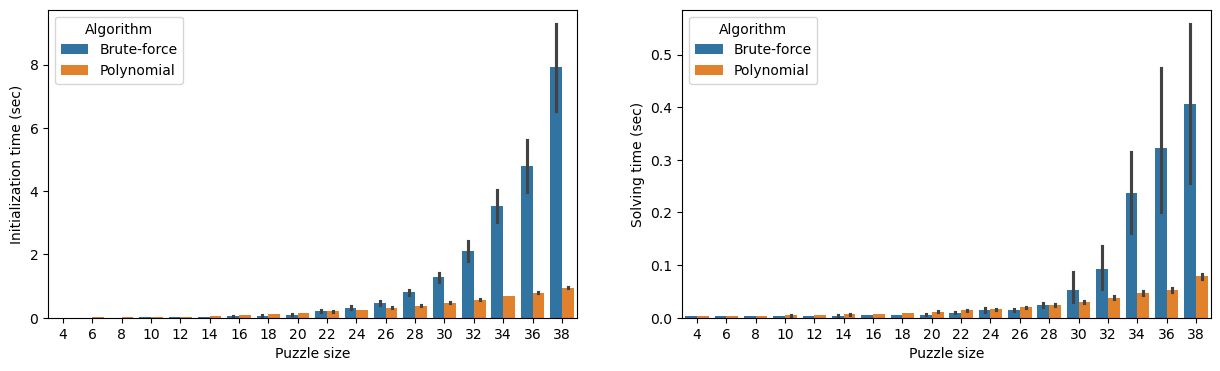
\includegraphics[scale=0.5]{bench.png}
  \centering
  \caption{Execution time for both algorithms proposed}
  \label{fig:bench}
\end{figure}

\dsa{Would be nice to have some benchmarking stats comparing different solutions}
\dsa{Check if time is spent in the setup of model or solving - do it in C and show that it gets better or even using Rust to write to file}

% \listoffigures

\end{document}
